% Compile with pdflatex to regenerate knowledge-base-schema.pdf.
\documentclass[tikz,border=2pt]{standalone}
\definecolor{ink}{HTML}{183643}
\definecolor{teal}{HTML}{19645E}
\definecolor{pale}{HTML}{EEF5F4}
\definecolor{grayblue}{HTML}{576974}
\begin{document}
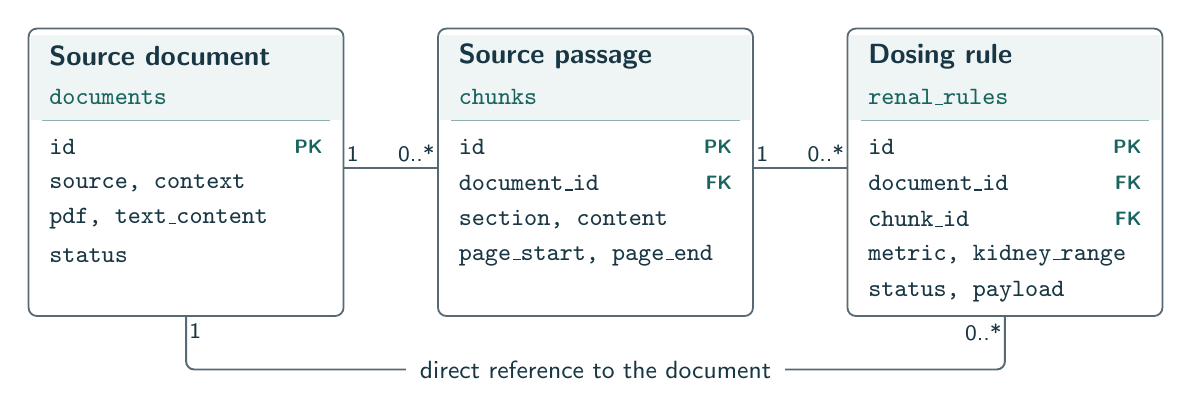
\begin{tikzpicture}[
  x=1cm,y=1cm,text=ink,font=\sffamily\small,
  box/.style={rounded corners=3pt,draw=grayblue,line width=.65pt},
  title/.style={anchor=west,font=\sffamily\bfseries\normalsize},
  name/.style={anchor=west,font=\ttfamily\small,text=teal},
  field/.style={anchor=west,font=\ttfamily\small},
  tag/.style={anchor=east,font=\sffamily\scriptsize\bfseries,text=teal},
  relation/.style={draw=grayblue,line width=.7pt},
  count/.style={font=\sffamily\footnotesize,inner sep=1pt}
]
  % Keep the table keys and their explanatory labels in separate columns.
  \foreach \x/\heading/\tablename in
    {0/Source document/documents,5.2/Source passage/chunks,10.4/Dosing rule/{renal\_rules}} {
    \begin{scope}[xshift=\x cm]
      \path[box,fill=white] (0,0) rectangle (4,3.65);
      \fill[pale] (.025,2.49) rectangle (3.975,3.57);
      \node[title] at (.14,3.30) {\heading};
      \node[name] at (.14,2.78) {\tablename};
      \draw[teal!50] (.17,2.48) -- (3.83,2.48);
      \node[field] at (.14,2.15) {id};
      \node[tag] at (3.86,2.15) {PK};
    \end{scope}
  }
  \node[field] at (.14,1.69) {source, context};
  \node[field] at (.14,1.23) {pdf, text\_content};
  \node[field] at (.14,.77) {status};

  \node[field] at (5.34,1.69) {document\_id};
  \node[tag] at (9.06,1.69) {FK};
  \node[field] at (5.34,1.23) {section, content};
  \node[field] at (5.34,.77) {page\_start, page\_end};

  \node[field] at (10.54,1.69) {document\_id};
  \node[tag] at (14.26,1.69) {FK};
  \node[field] at (10.54,1.23) {chunk\_id};
  \node[tag] at (14.26,1.23) {FK};
  \node[field] at (10.54,.77) {metric, kidney\_range};
  \node[field] at (10.54,.31) {status, payload};

  \foreach \a/\b in {4/5.2,9.2/10.4} {
    \draw[relation] (\a,1.88) -- (\b,1.88);
    \node[count,above right] at (\a,1.92) {1};
    \node[count,above left] at (\b,1.92) {0..*};
  }
  \draw[relation,rounded corners=3pt] (2,0) -- (2,-.68) -- (12.4,-.68) -- (12.4,0);
  \node[count,below right] at (2,-.06) {1};
  \node[count,below left] at (12.4,-.06) {0..*};
  \node[fill=white,inner xsep=5pt] at (7.2,-.68) {direct reference to the document};
\end{tikzpicture}
\end{document}
